\section{Transistorn}
\harec{a}{2.6}{2.6}
\label{transistorn}
\index{transistor}

\smallfig{images/cropped_pdfs/bild_2_2-16.pdf}{Schemasymboler}{fig:BildII2-16}

\subsection{Allmänt}

En transistor består av skikt av dopade halvledarelement som sammanfogats.
Vanligt är två N-skikt och ett mellanliggande P-skikt (NPN-transistor) eller två P-skikt och ett mellanliggande N-skikt (PNP-transistor).
Skikten är försedda med anslutningar.

Bild \ref{fig:BildII2-16} visar schemasymboler för de vanliga tran\-sistor\-typerna 
NPN-transistorer (bipolära), PNP-\-tran\-sistorer (bipolära) och
FET-transistorer (fälteffekt-).

\subsection{NPN-transistorer}
\harec{a}{2.6.1b}{2.6.1b}
\index{NPN-transistor}
\index{transistor!NPN}

Halvledarskikten kallas emitter (E), bas (B) och kollektor (C).

\smallfig[0.06]{images/cropped_pdfs/bild_2_6-37.pdf}{Transistor}{fig:BildII2-17a}

\noindent
Bild \ref{fig:BildII2-17a} visar en klassisk hålmonterad småsignaltransistor.

\subsubsection{Spärrzonerna}

\tallfig[0.30]{images/cropped_pdfs/bild_2_2-17.pdf}{Skikten i en bipolär transistor}{fig:BildII2-17}

Bild \ref{fig:BildII2-17} överst visar hur mellan skikten B och E respektive mellan B och C bildas zoner vars ledningsförmåga kan styras elektriskt över anslutningarna.

\begin{figure*}[p]
  \begin{center}
    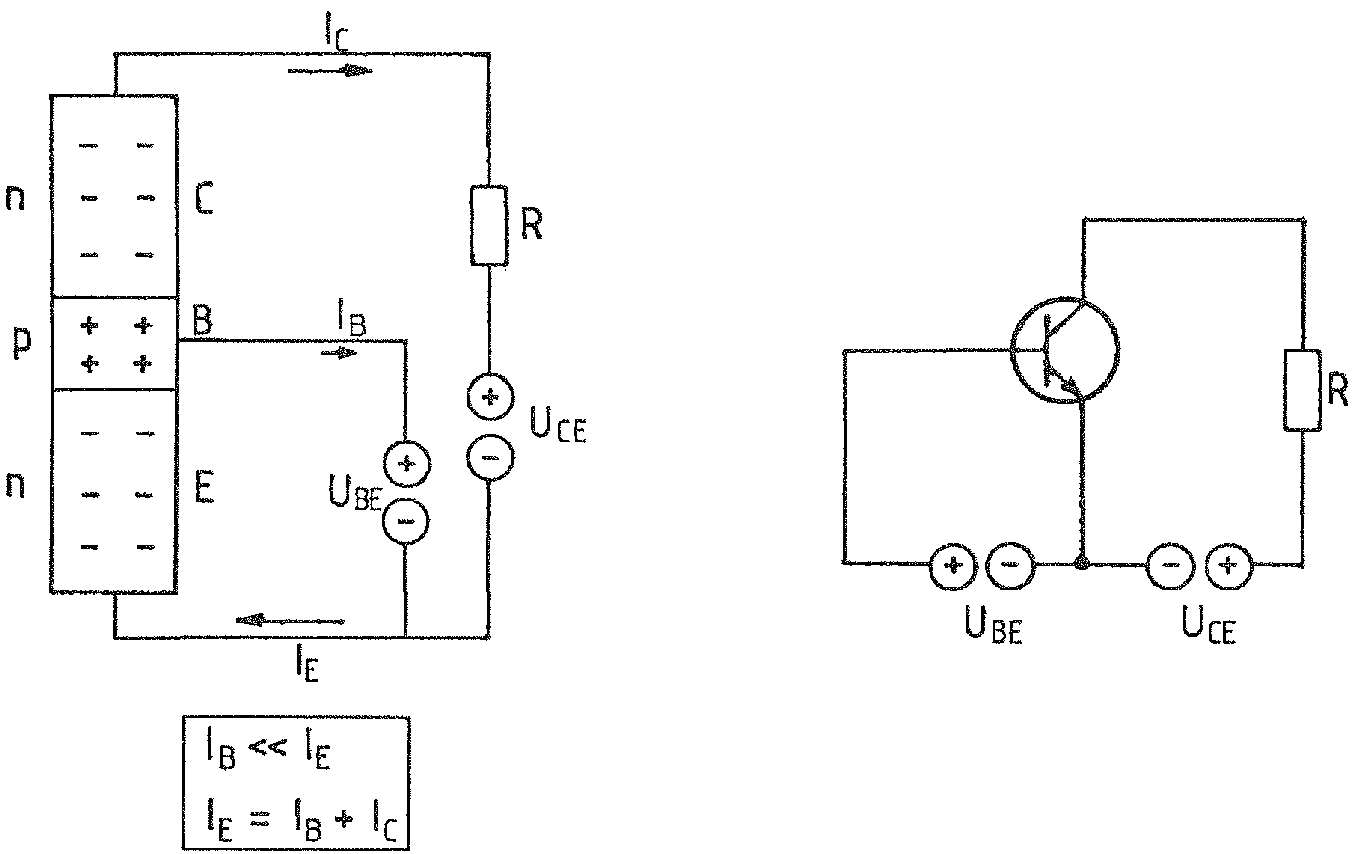
\includegraphics[width=0.66\textwidth]{images/cropped_pdfs/bild_2_2-18.pdf}
    \caption{Emitterkopplad transistor}
    \label{fig:BildII2-18}
  \end{center}
\end{figure*}

\begin{figure*}[p]
  \begin{center}
    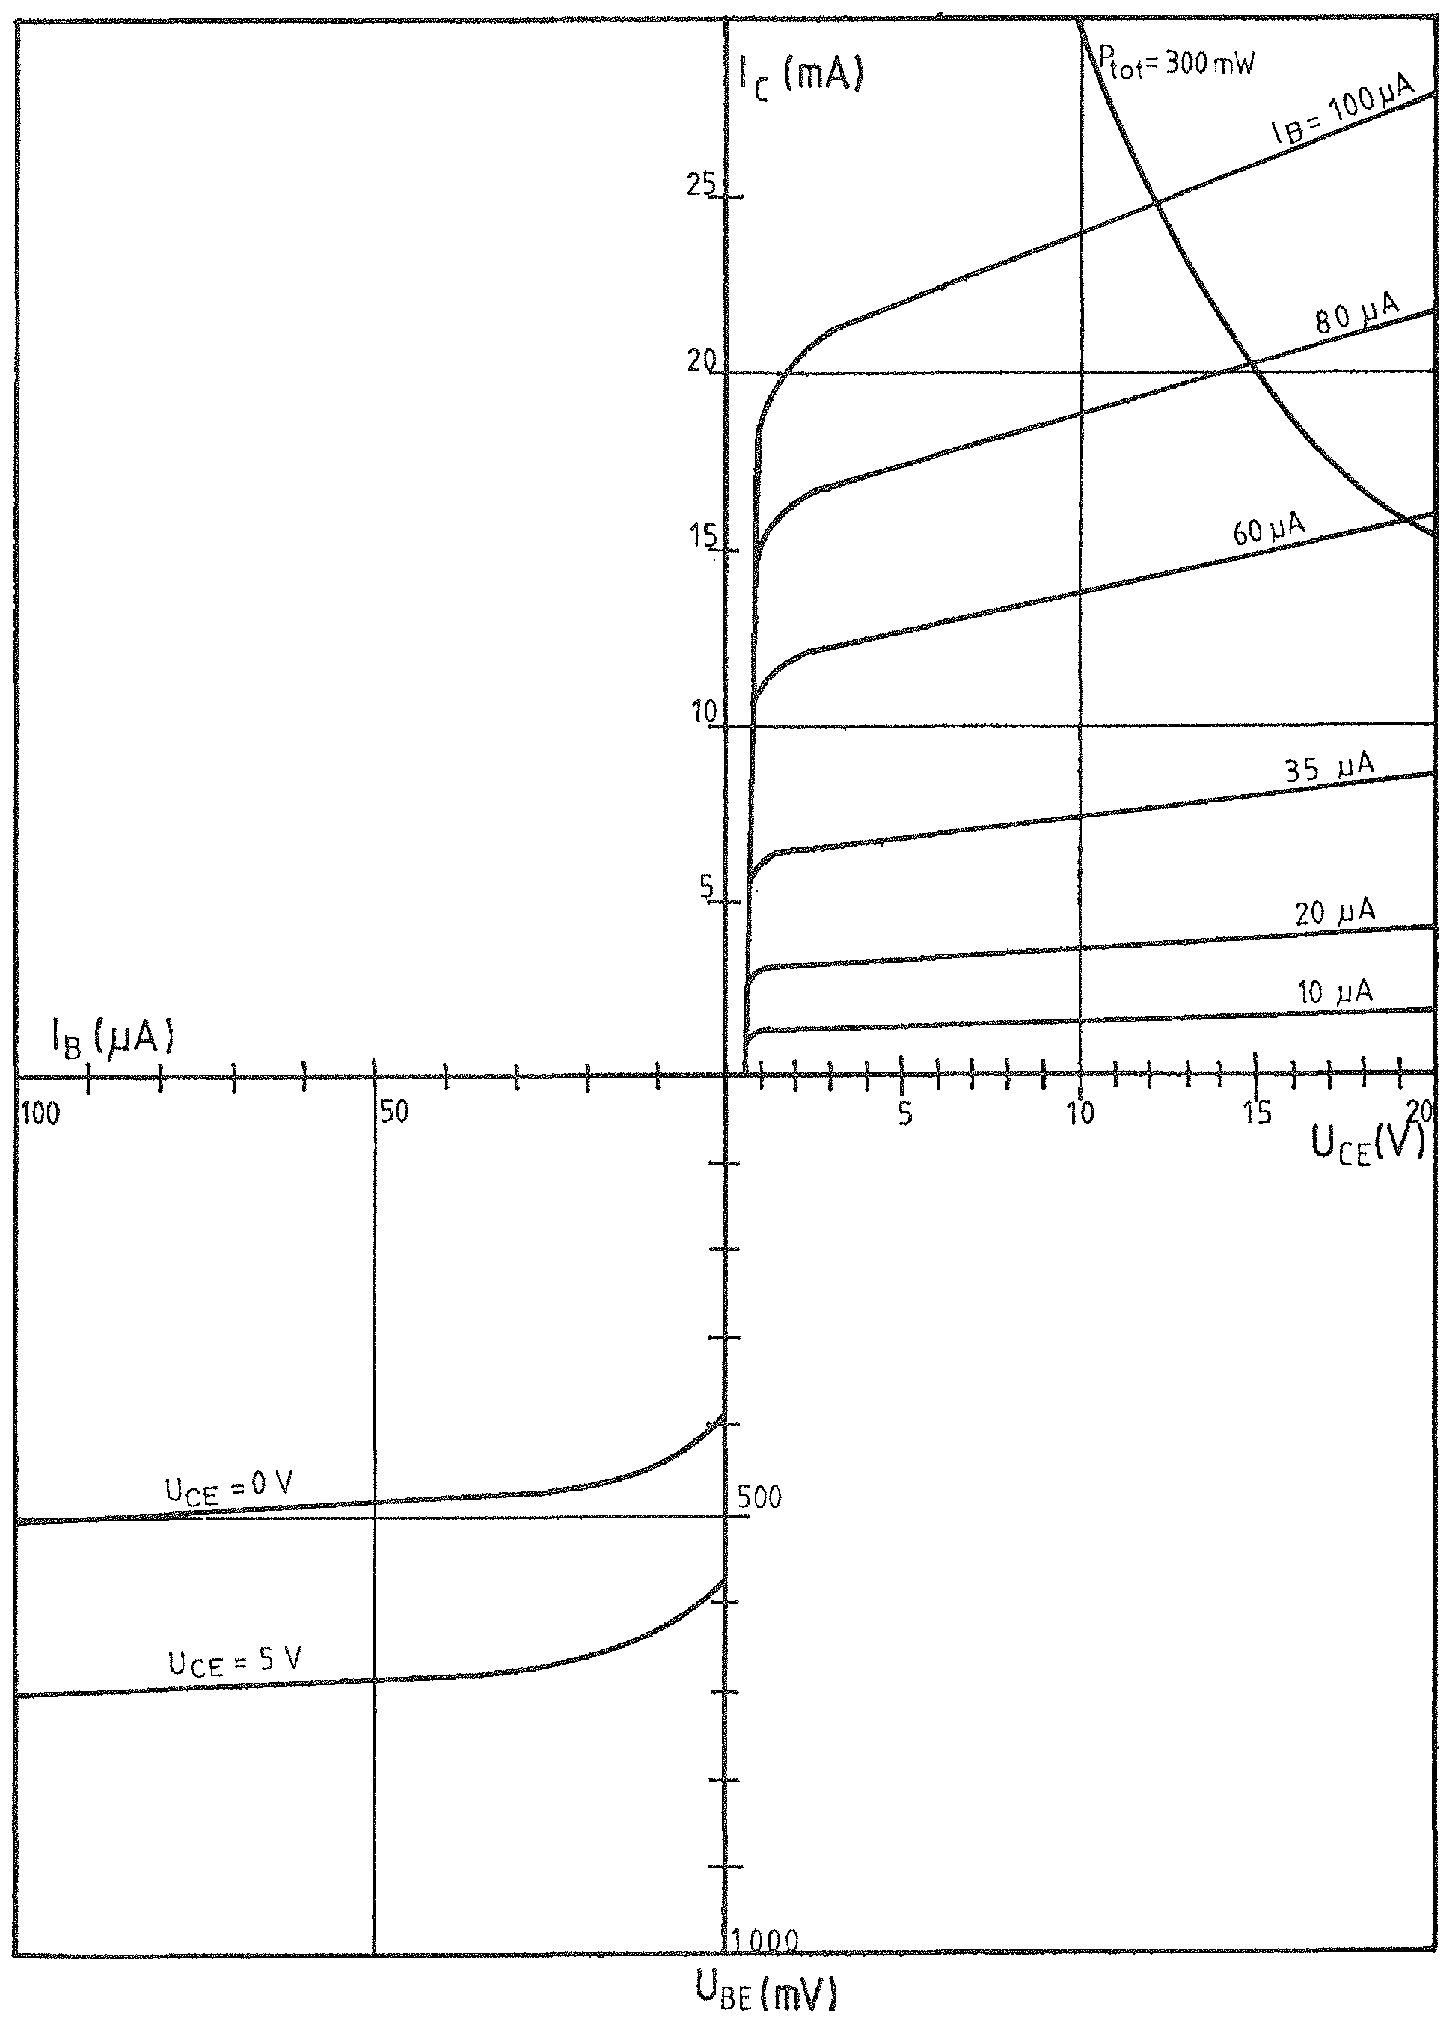
\includegraphics[width=0.66\textwidth]{images/cropped_pdfs/bild_2_2-19.pdf}
    \caption{Karaktäristika för transistor BC 107}
    \label{fig:BildII2-19}
  \end{center}
\end{figure*}

%%\clearpage

\subsubsection{Spänningskällan \(U_{BE}\)}

Bild \ref{fig:BildII2-17} mitten visar att mellan bas och emitter finns en diodsträcka.
När en positiv spänning läggs på basen och en negativ spänning på emittern polariseras diodsträckans spärrzon i passriktningen.
Spärrzonen upplöses då och det flyter en så kallad basström \(I_B\).

\subsubsection{Spänningskällan \(U_{CE}\)}

Bild \ref{fig:BildII2-17} nederst visar att när en positiv spänning läggs på kollektorn och en negativ spänning läggs på emittern polariseras diodsträckan i spärriktningen.
Spärrzonen förstärks då och det flyter ingen ström.

\subsubsection{Inverkan av både \(U_{BE}\) och \(U_{CE}\)}

Bild \ref{fig:BildII2-18} visar hur två spänningskällor \(U_{BE}\) och
\(U_{CE}\) ansluts till en emitterkopplad NPN-transistor.
Ur den starkt dopade emitterzonen strömmar elektronerna in i den svagt dopade
baszonen (spänning: \(U_{BE}\)).
De flesta elektronerna blir emellertid inte kvar i basen.
De stöter igenom det tunna basskiktet och når fram till
kollektorskiktet med spänningen \(U_{CE}\). Det flyter en kollektorström.

För strömmen \(I_E\) (emitterström), \(I_B\) (basström) och \(I_C\)
(kollektorström) gäller:
%%
\[I_E = I_B + I_C\quad \text{där} I_B \ll I_C\ (\ll \text{mycket mindre än})\]
%%
Kollektorströmmen \(I_C\) kan styras med basspänningen \(U_{BE}\).
En liten ändring i basspänningen ger stor förstärkande verkan i
kollektorströmmen.

\subsection{Förstärkningsfaktor}
\harec{a}{2.6.2}{2.6.2}
\index{förstärkningsfaktor!transistor}
\index{transistor!förstärkningsfaktor}

Om strömmen i ingångskretsen för en transistor ändras kan strömmen i utgångskretsen ändras mer. 
Vi får en förstärkning.

Av sambandet \(I_C = f(I_B)\) framgår strömförstärkningsfaktorn \(\beta\) eller
\(h_{FE}\) som är kvoten mellan ändringen i utgångsströmmen och ändringen i ingångsströmmen i
transistorns aktiva (linjära) område.

Bild \ref{fig:BildII2-19} visar ström-spänning-diagram för BC 107-transistorn för olika basströmmar.
För emitterkoppling gäller:
%%
\[h_{FE} = \dfrac{\Delta I_C}{\Delta I_B}~.\]
%%
\begin{tabular}{ll}
  \(h_{FE}\) & strömförstärkningsfaktorn \\
  \(\Delta I_C\)   & ändringen i kollektorströmmen \\
  \(\Delta I_B\)   & ändringen i basströmmen \\
\end{tabular}

\subsection{PNP-transistorer}
\harec{a}{2.6.1a}{2.6.1a}
\index{PNP-transistor}
\index{transistor!PNP}

Ersätter man de två N-skikten i en NPN-transistor med P-skikt och P-skiktet med
ett N-skikt så erhåller man en PNP-transistor.

Uppbyggnad, koppling och användning av en PNP-transistor motsvarar i övrigt den
för en NPN-transistor. Spänningskällorna måste emellertid ha motsatt polaritet.

\subsection{Fälteffekttransistorer}
\harec{a}{2.6.3}{2.6.3}
\index{fälteffekttransistor}
\index{transistor!fälteffekt}
\index{FET}
\index{transistor!FET}

\subsubsection{Allmänt}

\emph{Fälteffekttransistorer (FET)} har mycket hög ingångsimpedans och styrströmmen blir därför mycket svag.
Man säger därför att en FET är spänningsstyrd.

Även NPN- och PNP-transistorer -- bipolära transistorer -- styrs med spänning, men dessa typer har en relativt låg ingångsimpedans och därför högre styrström. Man säger därför att de är strömstyrda.

\smallfig[0.15]{images/cropped_pdfs/bild_2_2-20.pdf}{Schemasymbol för en FET}{fig:BildII2-20}

Bild \ref{fig:BildII2-20} anger en schemasymbol för en FET.

Fälteffekttransistorn har tre anslutningar, source (S), drain (D) och gate (G).

\smallfig[0.25]{images/cropped_pdfs/bild_2_2-21.pdf}{Skikten i en N-kanal FET}{fig:BildII2-21}

\subsubsection{Fälteffekttransistorns uppbyggnad}

Bild \ref{fig:BildII2-21} visar ett N-ledande skikt (även kallat N-kanal) med
anslutningarna S och D anslutna till respektive ändar av skiktet.
N-kanalen passerar mellan två P-ledande skikt förbundna med styrelektroden G.

När en spärrspänning läggs mellan G och S breder spärrskikten ut sig och N-kanalen blir trängre.
Läggs en negativ spänning på S och en positiv spänning på D, kommer en ström att flyta i N-kanalen.
Strömmens styrka kan påverkas med spänningen på G.

En liten spänningsändring \(\Delta U_{GS}\) medför stor ändring av strömmen
\(\Delta I_{GS}\) i N-kanalen. Detta innebär förstärkning.

\smallfig[0.25]{images/cropped_pdfs/bild_2_2-22.pdf}{Skikten i en N-kanal MOSFET}{fig:BildII2-22}

\index{MOSFET}
\index{transitor!MOSFET}

Bild \ref{fig:BildII2-22} visar skikten i en N-kanal MOSFET.

I en MOSFET (eng. \emph{Metal Oxide Semicoductor Field Effect Transistor}) är G-elektroden isolerad med ett kiseloxidskikt, trots att namnet förespeglar ett metalloxidskikt. Funktionssättet är samma som för en FET.
Drainströmmen kan ökas eller minskas med hjälp av en positiv respektive negativ spänning på G.

\subsubsection{Resistansen mellan gate och source}

För att erhålla en förstärkning med en FET sätter man in en resistor \(R_0\) i drainströmkretsen.
Över resistorn uppstår då spänningsändringar i proportion med strömändringarna.

För att fastställa viloströmmen och därmed arbetspunkten för samma transistor sätter man in en resistor \(R_S\) i sourceströmkretsen.
Storleken på sourceresistorn ger sig av önskad gateförspänning \(-U_{GS}\).
%%
\[R_S = \dfrac{-U_{GS}}{I_D}~.\]

\smallfig{images/cropped_pdfs/bild_2_2-23.pdf}{Karaktäristik för N-kanal FET}{fig:BildII2-23}

\subsection{Sambandet drain-ström och spänning}

%%Bild \ref{fig:BildII2-23} visar karaktäristiken för en N-kanals-FET.
För att beskriva en FET använder man sig av karaktäristiska kurvor (bild \ref{fig:BildII2-23}).
Vi har redan presenterat bipolära transistorers in- och utgångsegenskaper i kurvform.
Eftersom ingångsströmmen (gateströmmen) i en FET är praktiskt taget noll, är en sådan kurva utan praktisk mening.
I stället framställer man grafiskt sammanhanget mellan styrspänningen
\(U_{GS}\) och utgångsströmmen (drainströmmen \(I_D\)).
Eftersom det finns N-kanals-FET och P-kanals-FET så skiljer sig polariteten på \(U_{GS}\) mellan dessa båda typer.
